% begin module continuous-def
\begin{frame}
\frametitle{Continuity}
\begin{itemize}
\item<1-> Let $f$ be a function and $a$ be a point in its domain.
\item<2-> Suppose $\lim\limits_{x\rightarrow a}f(x)$ exists.
\end{itemize}
\uncover<3->{
\begin{definition}[Continuous at a Number]
We say that $f$ is continuous at $a$ if
\[
\lim_{x\rightarrow a}f(x) = f(a) .
\]
\end{definition}
}
\begin{center}
\psset{xunit=1cm, yunit=1cm}
\begin{pspicture}(-1, -0.5)(4,3.1) 
\psaxes[ticks=none, labels=none]{<->}(0,0)(-0.5,-0.5)(4,3)
%Function formula: 1/2 (1/2 x)^{3}+1/8 (1/2 x)^{4}- (1/2 x)^{2}+1 
\psplot[linecolor=red, plotpoints=1000]{-0.5}{4}{x 0.5 mul 4 exp 0.125 mul x 0.5 mul 2 exp -1 mul add x 0.5 mul 3 exp 0.5 mul add 1 add }
\end{pspicture} 
\end{center}
%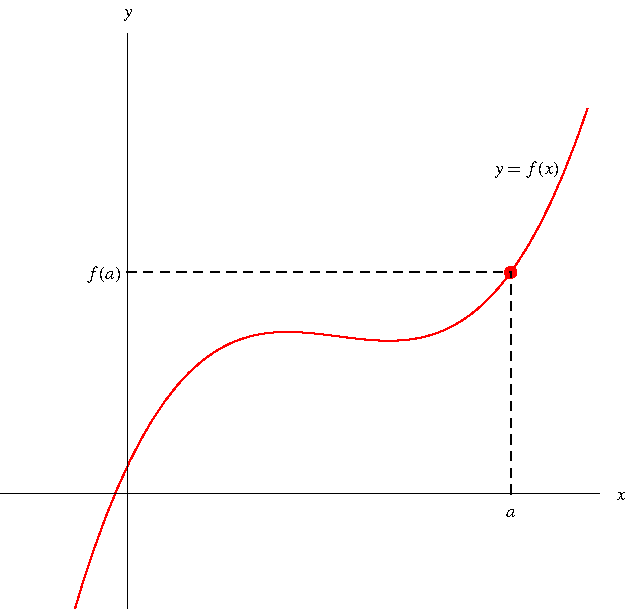
\includegraphics[height=4.5cm]{continuity/pictures/02-05-continuous.pdf}%
\end{frame}
% end module continuous-def

